\chapter{Modellentwicklung}\label{ch:modellentwicklung}

In diesem Kapitel wird die systematische Herangehensweise behandelt, mit der die Simulationsumgebung sukzessive erweitert wurde. Dabei ist nachvollziehbar aufbereitet, welche Informationen der Regelung und Steuerung im jeweiligen Schritt zu Verfügung stehen.

\section{Modellübersicht}

Für die Simulation werden drei verschiedene Modelle betrachtet. Zum einen das Modell, welches das physikalische Verhalten der Betonpumpe abbilden soll und zum anderen die Modelle, die dem Entwurf der Regelung und der Vorsteuerung zugrunde liegen. Alle Modell können entweder vollständig oder unvollständig aktuierte Eigenschaft aufweisen. Die Möglichkeit einen Stelleingriff auf jedes betrachtete Gelenk ausüben zu können, bedeutet dabei, dass es sich um ein vollständig aktuiertes Modell handelt. Bei unvollständig aktuierten Modellen werden zusätzlich Gelenke integriert, die das dynamische Verhalten verursachen, welches bei realen Betonpumpen beobachtet werden kann.\\

\begin{table}[htbp]
	\centering
	\caption{Mögliche Modellkombinationen}
	\label{tab:Modellübersicht}
	\begin{tabular}{llll}
		Fall & Modell der Simulation & Entwurfsmodell des  & Entwurfsmodell der\\
		&						& Reglers			& Steuerung\\
		\toprule
		1.& vollst. akt. & vollst. akt. & vollst. akt.\\
		2.& unvollst. akt. & vollst. akt. & vollst. akt.\\
		3.& unvollst. akt. & unvollst. akt. & vollst. akt.\\
		4.& unvollst. akt. & unvollst. akt. & unvollst. akt.\\
		\bottomrule\\
	\end{tabular}
\end{table}

In Tabelle \ref{tab:Modellübersicht} sind alle möglichen Modellkombinationen aufgelistet. In der folgenden Betrachtung wird ein exemplarischer Ausleger betrachtet, welcher aus zwei Gliedern besteht. Der Implementierungsaufwand nimmt zu, je mehr unvollständig aktuierte Modelle verwendet werden.


\section{Alle Modelle vollständig aktuiert (1. Fall)}

Im ersten Fall gilt die Annahme, dass sehr massive steife Glieder verbaut wurden, wodurch von einem unelastischen Ausleger ausgegangen werden kann, bei dem Schwingungen vernachlässigt werden. Dadurch sind alle Gelenke vollständig aktuiert und der Regelungs- und Steuerungsentwurf vereinfacht sich.

\begin{figure}[h]
	\centering
	\input{Manipulatorvollakt.pdf_tex}
	\caption{Manipulator vollständig aktuiert}
	\label{fig:VollAkt}
\end{figure} 

In Abbildung \ref{fig:VollAkt} ist das physikalische Modell eines vollständig aktuierten Manipulators dargestellt. Der Winkel $\theta_{11}$ gibt die absolute Auslenkung des ersten Segmentes zur horizontalen Bezugsebene wider und der Winkel $\theta_{21}$ die Auslenkung des zweiten Segmentes relativ zum ersten.

\begin{equation} \label{eq:VollAkt}
\underbrace{\vect{M}(\vect{\theta})\vectdd{\theta}}_{\mbox{Trägheitsmoment}} + \underbrace{\vect{C}(\vect{\theta},\vectd{\theta})\vectd{\theta}}_{\begin{matrix}
	\mbox{Zentrifugal-,} \\ \mbox{Coriolismoment} \end{matrix}}+\underbrace{\vect{g}(\vect{\theta)}}_{\begin{matrix}
	\mbox{Gravitations-} \\ \mbox{einfluss} \end{matrix}}=\underbrace{\vect{\tau}}_{\begin{matrix}
	\mbox{Stell-} \\ \mbox{momente} \end{matrix}}
\end{equation}

Die Modellgleichung ist in (\ref{eq:VollAkt}) zusammengefasst. Die Gleichung ist für das Simulationsmodell, die Regelung und die Steuerung die selbe. Es ist sofort sichtbar, dass sich die Stellgrößen einfach aus einer geforderten Solltrajektorie von $\theta$ und ihren zeitlichen Ableitungen bis zur zweiten Ordnung berechnen lassen.

\section{Simulationsmodell unteraktuiert (2. Fall)}

Das Simulationsmodell bildet approximiert das reales Verhalten des Auslegers ab. Die Glieder sind elastisch, so dass ein schwingungsfähiges System vorliegt. Zu jedem Segment wird zusätzlich ein unaktuiertes Gelenk modelliert, welches die Dynamik verursacht.

\begin{figure}[h]
	\centering
	\input{Manipulatorunterakt.pdf_tex}
	\caption{Manipulator unvollständig aktuiert}
	\label{fig:UnterAkt}
\end{figure}   

In Abbildung \ref{fig:UnterAkt} ist der Manipulator aus Abbildung \ref{fig:VollAkt} mit zusätzlichen elastischen Gelenken modelliert. Die Winkel $\theta_{12}$ und $\theta_{22}$ geben die Durchbiegung der Segmente wider.

\begin{equation} \label{eq:UnterAkt}
\underbrace{\vect{M}(\vect{\theta})\vectdd{\theta}}_{\mbox{Trägheitsmomente}} + \underbrace{\vect{C}(\vect{\theta},\vectd{\theta})\vectd{\theta}}_{\begin{matrix}
\mbox{Zentrifugal-,} \\ \mbox{Coriolismomente} \end{matrix}}+\underbrace{\vect{K}(\vect{\theta},\vectd{\theta})}_{\begin{matrix}
\mbox{Elastische} \\ \mbox{Fesselungsmomente} \end{matrix}}+\underbrace{\vect{g}(\vect{\theta})}_{\begin{matrix}
\mbox{Gravitations-} \\ \mbox{einfluss} \end{matrix}}=\underbrace{\vect{\tau}}_{\begin{matrix}
\mbox{Antriebs-} \\ \mbox{momente} \end{matrix}} 
\end{equation} 

Gleichung (\ref{eq:UnterAkt}) hat durch die elastischen Gelenke zusätzlich einen Term $\vect{K}(\vect{\theta},\vectd{\theta})$, welcher die geschwindigkeitsabhängige Dämpfung und auslenkungsabhängige Federmoment in den Gelenken $\theta_{12}$ und $\theta_{22}$ beschreibt. Die Dimension der Gleichungen ist um zwei erhöht worden. % Alle benannten Kräfte sind im rotatorischen System in ihrer Wirkung als Momente aufzufassen.
Aufgrund der Modellierung gibt es nur bei jedem zweiten Gelenk, in diesem Fall bei $\theta_{11}$ und $\theta_{21}$, einen Stelleingriff. Die übrigen Gelenke $\theta_{12}$ und $\theta_{22}$ sind passiv.

Das Modell für die Regelung und Steuerung ist vollständig aktuiert. Daraus folgt eine Einzelgelenkregelung. Alle Einflüsse, die durch die unaktuierten Gelenke und die Verkopplung resultieren, werden als Störgröße behandelt.

\section*{Implementierung} 

Bevor die ersten Simulationsergebnisse diskutiert werden, wird an dieser Stelle die Struktur der Implementierung erläutert.

\begin{figure}[h]
	\centering
	\input{Implementierung.pdf_tex}
	\caption{Implementierung des Regelkreises}
	\label{fig:Implementierung}
\end{figure}

In Abbildung \ref{fig:Implementierung} ist die Anordnung der einzelnen Teile des Regelkreises dargestellt. Das unvollständig aktuierte Modell des Auslegers ist in \textquotedblleft Modell\textquotedblright \,hinterlegt. Die Gleichungen (\ref{eq:UnterAkt}) sind in der Form eines Zustandsraumes zu lösen. Die Zustandsgröße ist $\vect{x}=(\vect{\theta},\vectd{\theta})^T$, mit den Winkeln und den Winkelgeschwindigkeiten als Komponenten.

\begin{equation} \label{eq:ModZR}
\vectd{x}	=	\begin{pmatrix}
				\vect{x}_2 \\
				\vect{M}^{-1}(\vect{x}_{1})(\vect{\tau} - \vect{C}(\vect{x}_1,\vect{x}_2)\vect{x}_2 - \vect{g}(\vect{x}_1) - \vect{K}(\vect{x}_1,\vect{x}_2))
			\end{pmatrix}
\end{equation}

In Gleichung (\ref{eq:ModZR}) ist der Zustandsraum des zu simulierenden gewöhnlichen Differentialgleichungssystem erster Ordnung notiert. In der Ruhelage $\vect{x}^\mathrm{e}=(\vect{x}_1^\mathrm{e},0)^T$ kompensiert die Vorsteuerung den Gravitationseinfluss (Gleichung (\ref{eq:tauVor})) 

\begin{equation} \label{eq:tauVor}
\vect{\tau}_{\mathrm{Vorsteuerung}} = \vect{g}(\vect{x}_1^\mathrm{e})
\end{equation}

Der PD-Regler verstärkt den Regelfehler des Winkels und der Winkelgeschwindigkeit und gibt die Stellgröße auf das Modell als Eingang, so dass der tatsächliche Ausgang dem Sollverlauf entspricht. Stationäre Regelabweichungen sind bei diesem Ansatz möglich.

\section*{Beispiel}

Im Folgenden werden einige Simulationsergebnisse behandelt. Für die Ruhelage wurden die Winkel:


\begin{align*}
\theta_{11}^\mathrm{e}&=60^\circ\\
\theta_{21}^\mathrm{e}&=-90^\circ\\
\theta_{12}^\mathrm{e}&=0\\
\theta_{22}^\mathrm{e}&=0\\
\end{align*}

gewählt. In Abbildung \ref{fig:animation}, in Kapitel \ref{ch:Visualisierung}, ist die Ruhelage skizziert. Die Werte von $\vect{\theta}^e=\vect{x}_1^e$ entsprechen den Anfangswerten $\vect{x}_1(0)=\vect{\theta}^e$ zum Zeitpunkt $t=0$.

\begin{figure}[h]
\centering
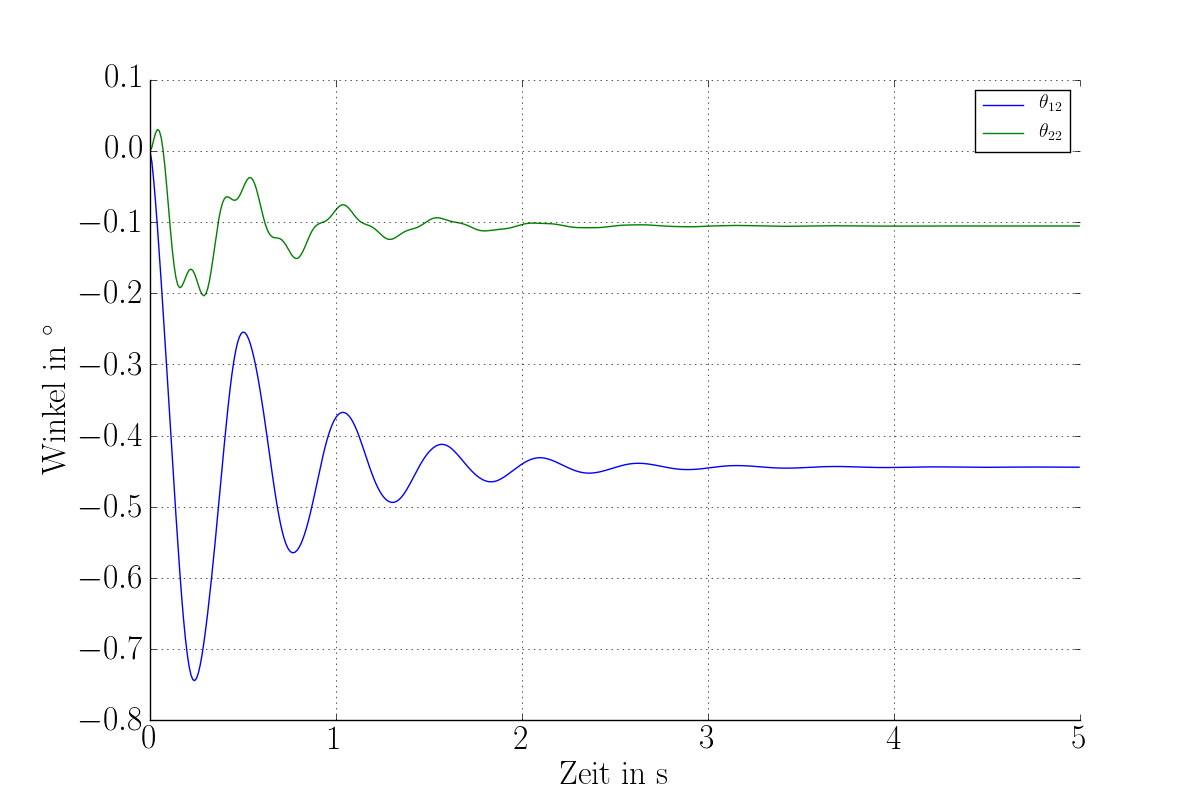
\includegraphics[width=1\linewidth]{RuhelageUnaktuierteGelenke.png}
\caption{Simulationsergebnisse unaktuierte Geleneke unvollständig aktuiertes Modell}
\label{fig:RuhelageUnaktuierteGelenke}
\end{figure}

In Abbildung \ref{fig:RuhelageUnaktuierteGelenke} ist der Winkelverlauf der unaktuierten Gelenke zu sehen. Zum Zeitpunkt $t=0$ haben diese Winkel keine Auslenkung. Innerhalb von zirka $3\,\si{s}$ schwingt sich der Ausleger in seine neue Ruhelage ein. Die Winkel sind negativ. Bei Betrachtung der Anordnung ist eine Durchbiegung, welche durch die zusätzlichen Gelenke modelliert ist, in mathematisch negative Richtung zu erwarten, da durch die Gravitationskraft ein Moment in der selben Richtung auf die Gelenke wirkt. Der Winkel $\theta_{12}$ hat eine größere Auslenkung, da der längere Teil des Auslegers durch seine höhere Masse ein stärkeres Moment ausübt.

\begin{figure}[h]
\centering
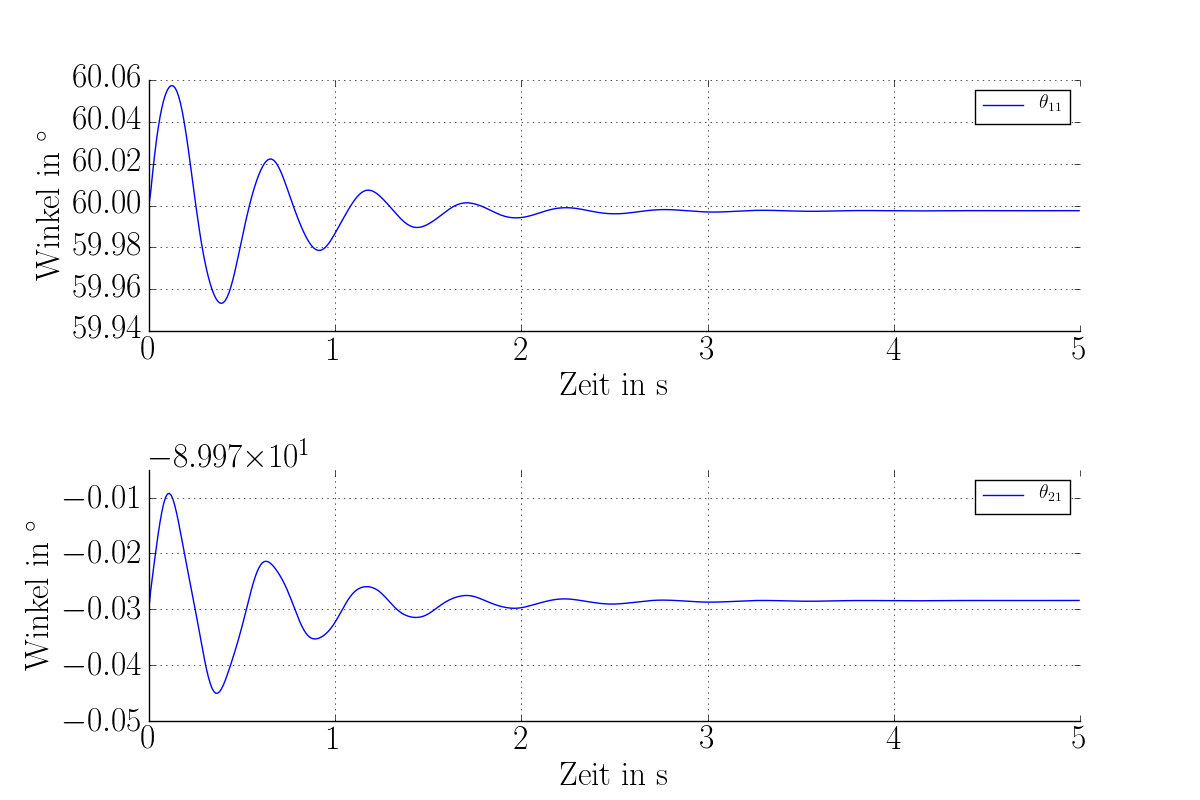
\includegraphics[width=1\linewidth]{RuhelageGelenkQ1Q2.png}
\caption{Simulationsergebnisse aktuierte Gelenke mit Einzelgelenkregelung}
\label{fig:RuhelageGelenkQ1Q2}
\end{figure}

Die Winkelverläufe der aktuierten Gelenke sind in Abbildung \ref{fig:RuhelageGelenkQ1Q2} gezeigt. Die Vorsteuerung kompensiert lediglich den Gravitationseinfluss, das heißt das Moment, welches dabei berechnet wird, ist über die gesamte Simulationsdauer konstant. Die Simulation startet nicht in der Ruhelage, für welche die Kompensation berechnet wurde. Damit entspricht dieser Wert auch nicht exakt dem notwendigen. Bei Beginn lenken die unaktuierten Gelenke im Uhrzeigersinn aus, wodurch ein leichter mathematisch positiver Ausschlag der aktuierten Gelenke verzeichnet wird. Die Regelung der einzelnen Gelenke wirkt dagegen. Nach dem Einschwingen verbleiben geringe stationäre Abweichungen, da nur ein PD-Regler verwendet wird, dessen Verstärkungen nicht optimal gewählt wurden. Die Simulationsergebnisse deuten an, dass die Einzelgelenkregelung in den Ruhelagen ausreichend ist, da nur geringe Abweichungen auftreten.
 
\section{Modell der Regelung unvollständig aktuiert (3. Fall)}

In diesem Fall kann durch die Kenntnis des unvollständig aktuierten Modells eine Ruhelage exakt berechnet werden. 

In unserem Beispiel ergeben sich folgende Werte:

\begin{align*}
\theta_{11}^e&=60^\circ\\
\theta_{21}^e&=-90^\circ\\
\theta_{12}^e&=-0,679^\circ\\
\theta_{22}^e&=-0,124^\circ\\
\end{align*}

Die tatsächliche Ruhelage der unaktuierten Gelenke befinden sich dadurch in der berechneten, wodurch daraus keine Störmomente auf die aktuierten Gelenke ausgeübt werden.

\begin{figure}[h]
\centering
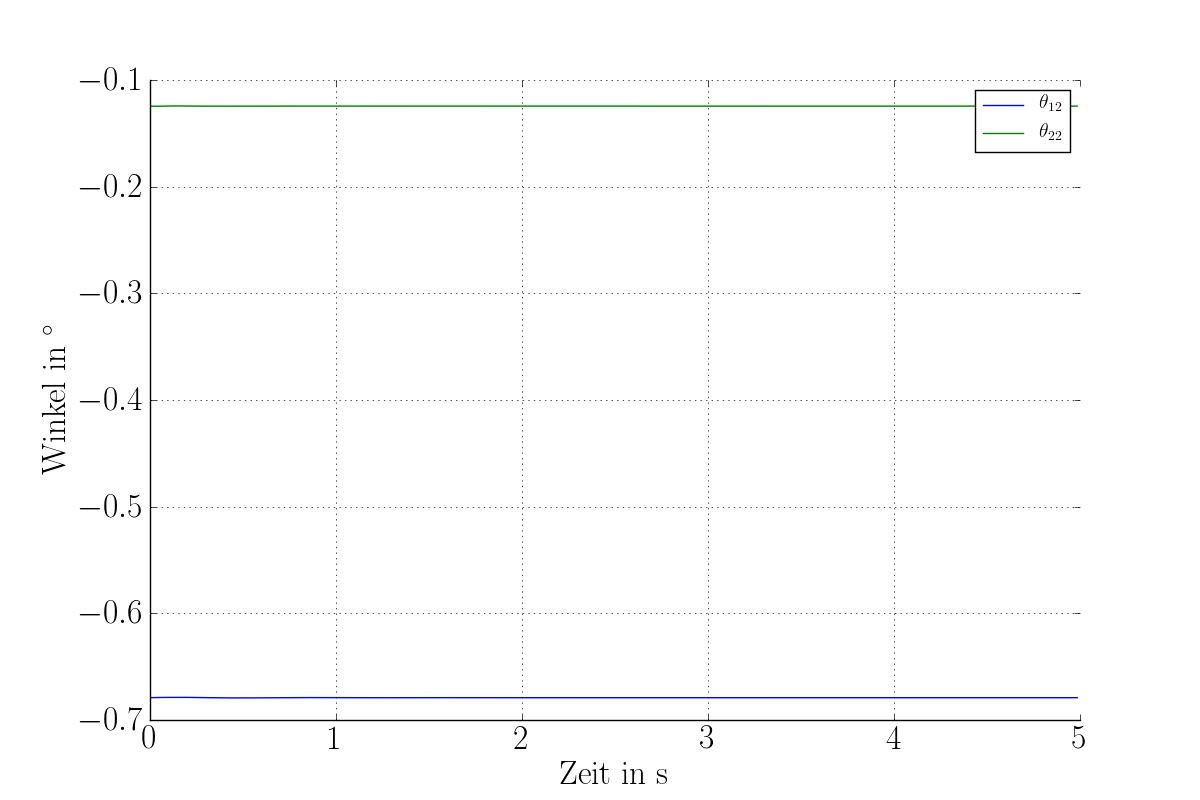
\includegraphics[width=1\linewidth]{lsgunvollvoll_unakt.png}
\caption{Simulationsergebisse unaktuierter Gelenke mit unvollständig aktuiertem Modell der Regelung}
\label{fig:unvollMod}
\end{figure}

Die Winkel $\theta_{12}$ und $\theta_{22}$ der unaktuierten Gelenke befinden sich sofort an der berechneten Position und sind konstant (Abbildung \ref{fig:unvollMod}). Dadurch treten sie nicht in Wechselwirkung mit den Winkeln der anderen Gelenken.

\begin{figure}[h]
\centering
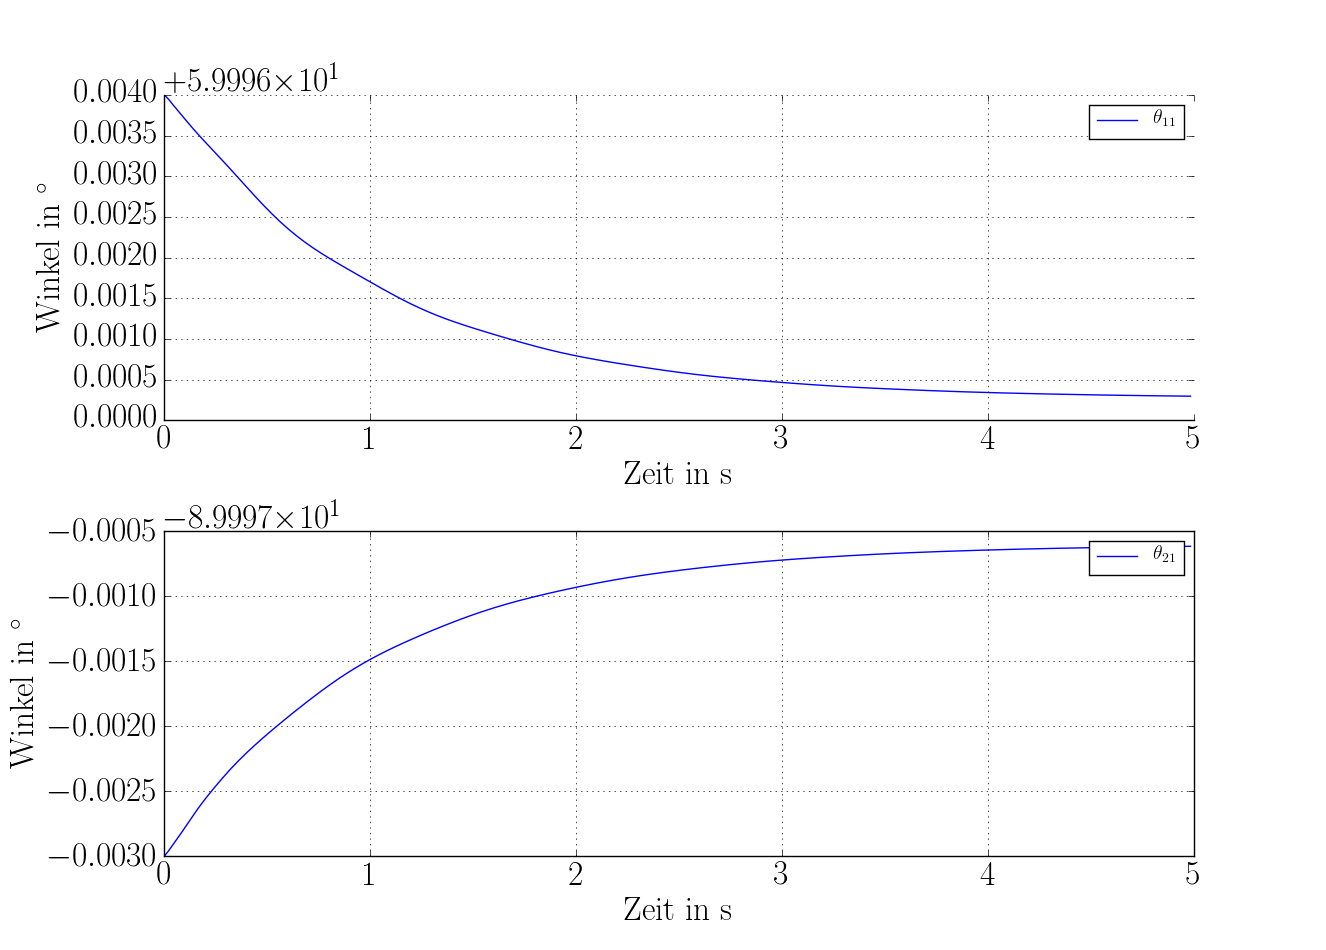
\includegraphics[width=1\linewidth]{lsgunvollvoll_akt.png}
\caption{Simulationsergebnisse der aktuierten Gelenke mit exakt berechneter Ruhelage}
\label{fig:lsgunvollvoll_unakt}
\end{figure}

Die Winkel $\theta_{11}$ und $\theta_{21}$ der aktuierten Gelenke erreichen ihre Sollposition nicht exakt, da die Steuerung noch das vollständig aktuierte Modell annimmt und die Stellgröße für die Ruhelage ungenau berechnet. Die stationäre Abweichung ist sehr gering und beträgt in diesem Beispiel zirka $0,0035^\circ$ (vgl. Abbildung \ref{fig:lsgunvollvoll_unakt}). Dieser Wert resultiert aus einer Simulation und ist in der  Praxis approximiert Null.

\newpage
\section{Alle Modelle unvollständig aktuiert (4. Fall)}

Bei der zusätzlichen Berücksichtigung eines unvollständigen Modells der Vorsteuerung ist die Kenntnis der Trajektorien aller Zustandskomponenten notwendig. Für eine Ruhelage sind diese mit akzeptablen Aufwand zu berechnen. Sofern ein Arbeitspunktübergang zwischen zwei Ruhelagen vollzogen werden soll, muss ein Randwertproblem gelöst werden. Die Lösung besteht aus Trajektorien, welche den Systemdifferentialgleichungen genügen und in gewünschtem Verhalten lösen. %Daraus ergibt sich beispielsweise, dass alle Winkel in der Ruhelage exakt dieser entsprechen.